
\chapter{Python for Scientific Computing}

\begin{flushright}
With material contributed by Perry Greenfield, Robert Jedrzejewski,
Vicki Laidler and John Hunter
\par\end{flushright}


\section{Who is using Python?}

The use of Python in scientific computing is as wide as the field
itself. A sampling of current work is provided here to indicate the
breadth of disciplines represented and the scale of the problems addressed.
The NASA Jet Propulsion Laboratory (JPL) uses Python as an interface
language to \textsc{FORTRAN} and C++ libraries which form a suite
of tools for plotting and visualization of spacecraft trajectory parameters
in mission design and navigation. The Space Telescope Science Institute
(STScI) uses Python in many phases of their pipeline: scheduling Hubble
data acquisitions, managing volumes of data, and analyzing astronomical
images \cite{BarrettEtal2004}. The National Oceanic Atmospheric Administration
(NOAA) uses Python for a wide variety of scientific computing tasks
including simple scripts to parse and translate data files, prototyping
of computational algorithms, writing user interfaces, web front ends,
and the development of models \cite{NOAA2000,BarkerHealy2001,ParkerHallBarker2001}.
At the Fundamental Symmetries Lab at Princeton University, Python
is used to efficiently analyze large data sets from an experiment
that searches for CPT and Lorentz Violation using an atomic magnetometer
\cite{Kornack2002,Kominis2003}. The Pediatric Clinical Electrophysiology
unit at The University of Chicago, which collects approximately 100\,GB
of data per week, uses Python to explore novel approaches to the localization
and detection of epileptic seizures \cite{HunterEtal2005}. The Enthought
Corporation is using Python to build customized applications for oil
exploration for the petroleum industry. At the world's largest radio
telescopes, e.g., Arecibo and the Green Bank Telescope, Python is
used for data processing, modelling, and scripting high-performance
computing jobs in order to search for and monitor binary and millisecond
pulsars in terabyte datasets \cite{Ransometal2004a,Ransom2005}. At
the Computational Genomics Laboratory at the Australian National University,
researchers are using Python to build a toolkit which enables the
specification of novel statistical models of sequence evolution on
parallel hardware \cite{Huttley2004,Butterfield2004}. Michel Sanner's
group at the Scripps Research Institute uses Python extensively to
build a suite of applications for molecular visualization and exploration
of drug/molecule interactions using virtual reality and 3D printing
technology\cite{Sanner2005a,Sanner2005b}. Engineers at Google use
Python in automation, control and tuning of their computational grid,
and use \texttt{SWIG} generated Python of their in-house C++ libraries
in virtually all facets of their work \cite{Beazley1998,Stein2005}.
Many other use cases -- ranging from animation at Industrial Light
and Magic, to space shuttle mission control, to grid monitoring and
control at Rackspace, to drug discovery, meteorology and air traffic
control -- are detailed in O'Reilly's two volumes of \emph{Python
Success Stories} \cite{PySuccess2002,PySuccess2005}.


\section{Advantages of Python}

\begin{quotation}
\textit{The canonical, \char`\"{}Python is a great first language\char`\"{},
elicited, \char`\"{}Python is a great last language!\char`\"{}} --
Noah Spurrier 
\end{quotation}
This quotation summarizes an important reason scientists migrate to
Python as a programming language. As a {}``great first language''
Python has a simple, expressive syntax that is accessible to the newcomer.
{}``Python as executable pseudocode'' reflects the fact that Python
syntax mirrors the obvious and intuitive pseudo-code syntax used in
many journals \cite{Strous2001}. As a great first language, it does
not impose a single programming paradigm on scientists, as Java does
with object oriented programming, but rather allows one to code at
many levels of sophistication, including BASIC/FORTRAN/Matlab style
procedural programming familiar to many scientists. Here is the canonical
first program {}``hello world'' in Python:

\noindent {\small \begin{verbatim}
# Python
print 'hello world'
\end{verbatim}}  Contrast the simplicity of that program with the complexity {}``hello
world'' in Java  {\small \begin{verbatim}
// java 
class myfirstjavaprog
{  
  public static void main(String args[])
  {
    System.out.println("Hello World!");
  }
} 
\end{verbatim}} 

\noindent In addition to being accessible to new programmers and scientists,
Python is powerful enough to manage the complexity of large applications,
supporting functional programming, object orienting programming, generic
programming and metaprogramming. That Python supports these paradigms
suggests why it is also a {}``great last language'': as one increases
their programming sophistication, the language scales naturally. By
contrast, commercial languages like Matlab and IDL, which also support
a simple syntax for simple programs do not scale well to complex programming
tasks.

The built-in Python data-types and standard library provide a powerful
platform in every distribution \cite{PyLibRef,Lundh2001}. The standard
data types encompass regular and arbitrary length integers, complex
numbers, floating point numbers, strings, lists, associative arrays,
sets and more. In the standard library included with every Python
distribution are modules for regular expressions, data encodings,
multimedia formats, math, networking protocols, binary arrays and
files, and much more. Thus one can open a file on a remote web server
and work with it as easily as with a local file \begin{verbatim}
# this 3 line script downloads and prints the yahoo web site
from urllib import urlopen
for line in urlopen('http://yahoo.com').readlines():
   print line
\end{verbatim}

Complementing these built-in features, Python is also readily extensible,
giving it a wealth of libraries for scientific computing that have
been in development for many years \cite{Dubois1996b,Dubois1996c}.
\texttt{Numeric Python} supports large array manipulations, math,
optimized linear algebra, efficient Fourier transforms and random
numbers. \texttt{scipy} is a collection of Python wrappers of high
performance FORTRAN code (eg LAPACK, ODEPACK) for numerical analysis
\cite{LAPACK}. \texttt{IPython} is a command shell ala Mathematica,
Matlab and IDL for interactive programming, data exploration and visualization
with support for command history, completion, debugging and more.
\texttt{Matplotlib} is a 2D graphics package for making publication
quality graphics with a Matlab compatible syntax that is also embeddable
in applications. \texttt{f2py}, \texttt{SWIG}, \texttt{weave}, and
\texttt{pyrex} are tools for rapidly building Python interfaces to
high performance compiled code, \texttt{MayaVi} is a user friendly
graphical user interface for 3D visualizations built on top of the
state-of-the-art Visualization Toolkit \cite{SchroederEtal2002}.
\texttt{pympi}, \texttt{pypar}, \texttt{pyro}, \texttt{scipy.cow},
and \texttt{pyxg} are tools for cluster building and doing parallel,
remote and distributed computations. This is a sampling of general
purpose libraries for scientific computing in Python, and does not
begin to address the many high quality, domain specific libraries
that are also available.

All of the infrastructure described above is open source software
that is freely distributable for academic and commercial use. In both
the educational and scientific arenas, this is a critical point. For
education, this platform provides students with tools that they can
take with them outside the classroom to their homes and jobs and careers
beyond. By contrast, the use commercial tools such as Matlab and IDL
limits access to major institutions. For scientists, the use of open
source tools is consistent with the scientific principle that all
of the steps in an analysis or simulation should be open for review,
and with the principle of reproducible research \cite{BuckheitDonoho1995}.


\section{Mixed Language Programming}

The programming languages of each generation evolve in part to fix
the problems of those that came before \cite{BerginEtal1996}. \textsc{FORTRAN},
the original high level language of scientific computing \cite{Rosen1967},
was designed to allow scientists to express code at a level closer
to the language of the problem domain. \textsc{ALGOL} and its successor
Pascal, widely used in education in the 1970s, were designed to alleviate
some of the perceived problems with \textsc{FORTRAN} and to create
a language with a simpler and more expressive syntax \cite{Backus1963,Naur1963}.
Object oriented programming languages evolved to allow a closer correspondence
between the code and the physical system it models \cite{GoldbergRobson1989},
and C++ provided a relatively high performance object orientated implementation
compatible with the popular C programming language \cite{Stroustrup1994,Stroustrup2000}.
But implementing object orientation efficiently requires programmers
stay close to the machine, managing memory and pointers, and this
created a lot of complexity in programs while limiting portability.
Interpreted languages such as Tcl, Perl, Python, and Java evolved
to manage some of the low-level and platform specific details, making
programs easier to write and maintain, but with a performance penalty
\cite{Ousterhout1998,ArnoldEtal2005}. For many scientists, however,
pure object oriented systems like Java are unfamiliar, and languages
like Matlab and Python provide the safety, portability and ease of
use of an interpreted language without imposing an object oriented
approach to coding \cite{VanRossumDrake2003,HanselmanLittlefield2004}.

The result of these several decades is that there are many platforms
for scientific computing in use today. The number of man hours invested
in numerical methods in \textsc{FORTRAN}, visualization libraries
in C++, bioinformatics toolkits in Perl, object frameworks in Java,
domain specific toolkits in Matlab, etc\dots requires an approach
that integrates this work. Python is the language that provides maximal
integration with other languages, with tools for transparently and
semi-automatically interfacing with \textsc{FORTRAN}, C, C++, Java,
.NET, Matlab, and Mathematica code \cite{Hugunin1997,Beazley1998}.
In our view, the ability to work seamlessly with code from many languages
is the present and the future of scientific computing, and Python
effectively integrates these languages into a single environment.


\section{Getting started}

We'll get started with python by introducing arrays and plotting by
working with a simple ASCII text file \texttt{mydata.dat} of two columns;
the first column contains the times that some measurement was acquired,
and the second column are the sampled voltages at that time. The file
looks like

\begin{lyxcode}
0.0000~0.4911

0.0500~0.5012

0.1000~0.7236

0.1500~1.1756

...~and~so~on
\end{lyxcode}
\noindent While it would be easy enough to process this file by writing
a python function to do it, there is no need to, since the matplotlib
pylab module has a matlab-compatible l\texttt{oad} function for loading
ASCII array data (Figure \ref{fig:load_ascii}). To complete these
exercises, you should have ipython and matplotlib installed, and start
ipython in pylab mode with 

\begin{lyxcode}
>~ipython~-pylab

%
\begin{figure}
\begin{centering}
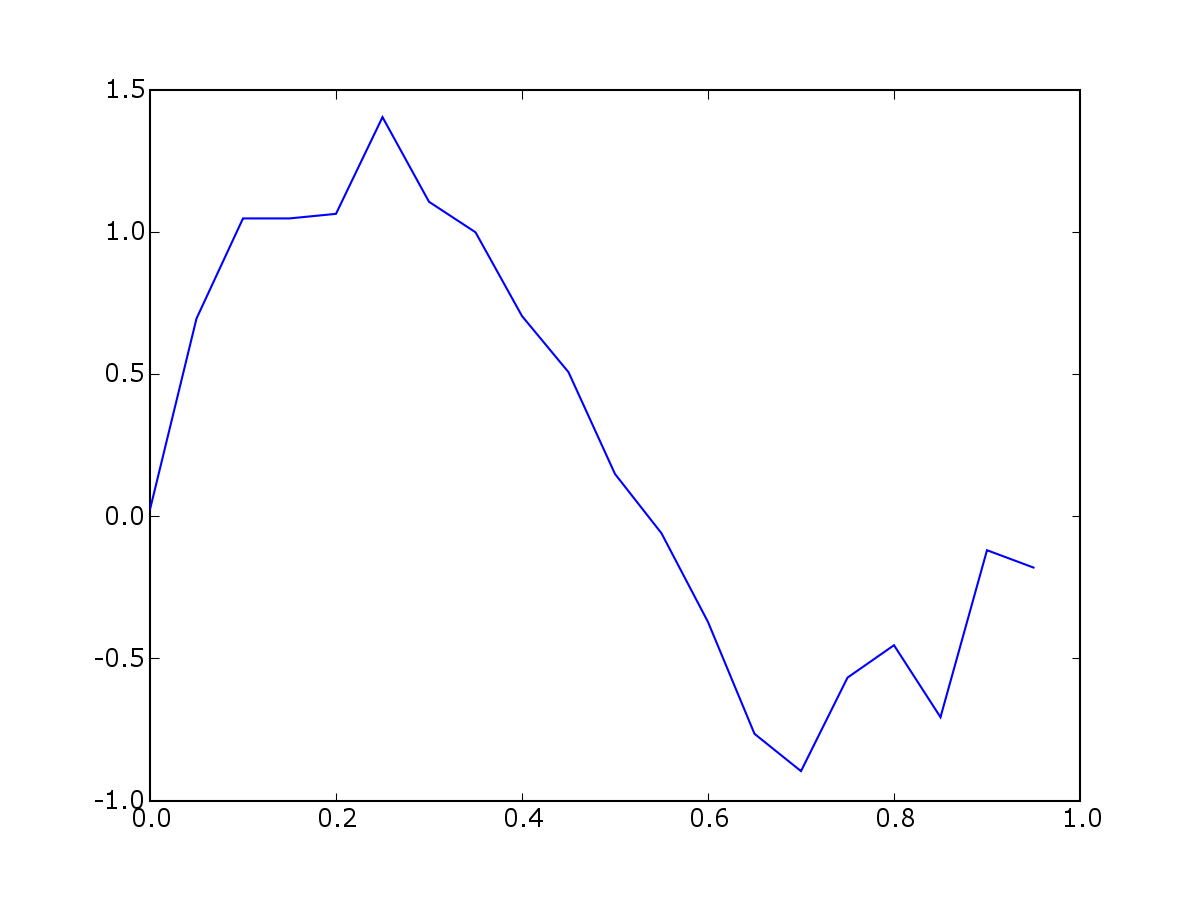
\includegraphics[width=4in]{fig/load_ascii}
\par\end{centering}

\caption{\label{fig:load_ascii}Loading \texttt{ASCII} data and displaying
with \texttt{plot}}

\end{figure}

\end{lyxcode}
\lstinputlisting[caption={Loading an ASCII text file and plotting the columns}]{snippets/load_data.ipy}



It is also easy to load data from binary files. In the example below,
we have some image data in raw binary string format. The image is
256x256 pixels, and each pixel is a 2 byte integer. We read this into
a string using python's \texttt{file} function -- the 'rb' flag says
to open the file in \texttt{read/binary} mode. We can then use the
numerix \texttt{fromstring} method to convert this to an array, passing
the type of the data (\texttt{Int16}) as an argument. We reshape the
array by changing the array shape attribute to 256 by 256, and pass
this off to the matplotlib pylab command \texttt{imshow} for plotting.
matplotlib has a number of colormaps, and the default one is jet;
the data are automatically normalized and colormaps producing the
image in Figure \ref{fig:array_hothead}

\lstinputlisting[caption={Loading an binary image data and plotting it in matplotlib}]{snippets/load_binary.ipy}



%
\begin{figure}
\begin{centering}
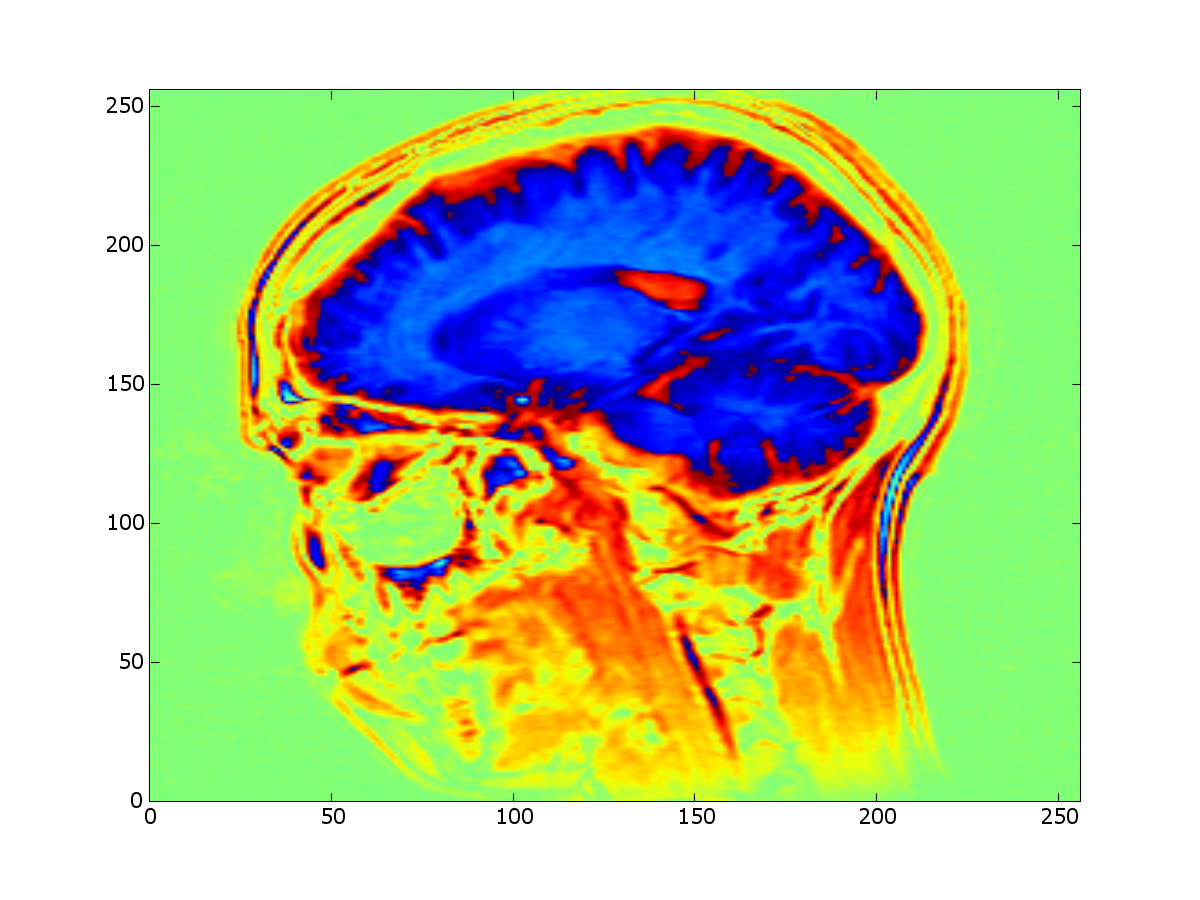
\includegraphics[width=4in]{fig/hothead}
\par\end{centering}

\caption{\label{fig:array_hothead}Loading binary image data and displaying
with \texttt{imshow}}

\end{figure}



\section[Arrays]{An Introduction to Arrays}


\subsection{Creating arrays}

There are a few different ways to create arrays besides modules that
obtain arrays from data files such

\begin{lyxcode}
>\,{}>\,{}>~x~=~zeros((20,30))
\end{lyxcode}
creates a 20x30 array of zeros (default integer type; details on how
to specify other types will follow). Note that the dimensions ({}``shape''
in numarray parlance) are specified by giving the dimensions as a
comma-separated list within parentheses. The parentheses aren't necessary
for a single dimension. As an aside, the parentheses used this way
are being used to specify a Python tuple; more will be said about
those in a later tutorial. For now you only need to imitate this usage.

Likewise one can create an array of 1's using the \texttt{ones()}
function.

The \texttt{arange()} function can be used to create arrays with sequential
values. E.g.,

\begin{lyxcode}
>\,{}>\,{}>~arange(10)

array({[}0,~1,~2,~3,~4,~5,~6,~7,~8,~9])
\end{lyxcode}
Note that that the array defaults to starting with a 0 value and does
not include the value specified (though the array does have a length
that corresponds to the argument)

Other variants:

\begin{lyxcode}
>\,{}>\,{}>~arange(10.)

array({[}~0.,~1.,~2.,~3.,~4.,~5.,~6.,~7.,~8.,~9])

>\,{}>\,{}>~arange(3,10)

array({[}3,~4,~5,~6,~7,~8,~9])

>\,{}>\,{}>~arange(1.,~10.,~1.1)~\#~note~trickiness

array({[}1.~,~2.1,~3.2,~4.3,~5.4,~6.5,~7.6,~8.7,~9.8])
\end{lyxcode}
Finally, one can create arrays from literal arguments:

\begin{lyxcode}
>\,{}>\,{}>~print~array({[}3,1,7])

{[}3~1~7]

>\,{}>\,{}>~print~array({[}{[}2,3],{[}4,4]])

{[}{[}2~3]

~{[}4~4]]
\end{lyxcode}
The brackets, like the parentheses in the zeros example above have
a special meaning in Python which will be covered later (Python lists).
For now, just mimic the syntax used here.


\subsection{Array numeric types}

numarray supports all standard numeric types. The default integer
matches what Python uses for integers, usually 32 bit integers or
what numarray calls \texttt{Int32}. The same is true for floats, i.e.,
generally 64-bit doubles called \texttt{Float64} in numarray. The
default complex type is \texttt{Complex64}. Many of the functions
accept a type argument. For example

\begin{lyxcode}
>\,{}>\,{}>~zeros(3,~Int8)~\#~Signed~byte

>\,{}>\,{}>~zeros(3,~type=UInt8)~\#~Unsigned~byte

>\,{}>\,{}>~array({[}2,3],~type=Float32)

>\,{}>\,{}>~arange(4,~type=Complex64)
\end{lyxcode}
The possible types are \texttt{Int8, UInt8, Int16, UInt16, Int32,
UInt32, Int64, UInt64, Float32, Float64, Complex32, Complex64.} To
find out the type of an array use the .type() method. E.g.,

\begin{lyxcode}
>\,{}>\,{}>~arr.type()

Float32
\end{lyxcode}
To convert an array to a different type use the \texttt{astype()}
method, e.g,

\begin{lyxcode}
>\,{}>\,{}>~a~=~arr.astype(Float64)
\end{lyxcode}

\subsection{Printing arrays}

Interactively, there are two common ways to see the value of an array.
Like many Python objects, just typing the name of the variable itself
will print its contents (this only works in interactive mode). You
can also explicitly print it. The following illustrates both approaches:

\begin{lyxcode}
>\,{}>\,{}>~x~=~arange(10)

>\,{}>\,{}>~x

array({[}0,~1,~2,~3,~4,~5,~6,~7,~8~9])

>\,{}>\,{}>~print~x

{[}0~1~2~3~4~5~6~7~8~9]
\end{lyxcode}
By default the array module limits the amount of an array that is
printed out (to spare you the effects of printing out millions of
values). For example:

\begin{lyxcode}
>\,{}>\,{}>~x~=~arange(1000000)

print~x

{[}~~~~0~~~~~1~~~~~2~...,~999997~999998~999999]
\end{lyxcode}

\subsection{Indexing 1-D arrays}

As with IDL and Matlab, there are many options for indexing arrays.

\begin{lyxcode}
>\,{}>\,{}>~x~=~arange(10)

>\,{}>\,{}>~x

array({[}0,~1,~2,~3,~4,~5,~6,~7,~8,~9])
\end{lyxcode}
Simple indexing:

\begin{lyxcode}
>\,{}>\,{}>~x{[}2]~\#~3rd~element

2
\end{lyxcode}
Indexing is 0-based. The first value in the array is \texttt{x{[}0]}

Indexing from end:

\begin{lyxcode}
>\,{}>\,{}>~x{[}-2]~\#~-1~represents~the~last~element,~-2~next~to~last...

8
\end{lyxcode}
Slices

To select a subset of an array:

\begin{lyxcode}
>\,{}>\,{}>~x{[}2:5]

array({[}2,~3,~4])
\end{lyxcode}
Note that the upper limit of the slice is not included as part of
the subset! This is viewed as unexpected by newcomers and a defect.
Most find this behavior very useful after getting used to it (the
reasons won't be given here). Also important to understand is that
slices are views into the original array in the same sense that references
view the same array. The following demonstrates:

\begin{lyxcode}
>\,{}>\,{}>~y~=~x{[}2:5]

>\,{}>\,{}>~y{[}0]~=~99

>\,{}>\,{}>~y

array({[}99,~3,~4])

>\,{}>\,{}>~x

array({[}0,~1,~99,~3,~4,~5,~6,~7,~8,~9])
\end{lyxcode}
Changes to a slice will show up in the original. If a copy is needed
use \texttt{x{[}2:5].copy()}

Short hand notation

\begin{lyxcode}
>\,{}>\,{}>~x{[}:5]~\#~presumes~start~from~beginning

array({[}~0,~1,~99,~3,~4])

>\,{}>\,{}>~x{[}2:]~\#~presumes~goes~until~end

array({[}99,~3,~4,~5,~6,~7,~8,~9])

>\,{}>\,{}>~x{[}:]~\#~selects~whole~dimension

array({[}0,~1,~99,~3,~4,~5,~6,~7,~8,~9])
\end{lyxcode}
Strides:

\begin{lyxcode}
>\,{}>\,{}>~x{[}2:8:3]~\#~Stride~every~third~element

array({[}99,~5])
\end{lyxcode}
Index arrays:

\begin{lyxcode}
>\,{}>\,{}>~x{[}{[}4,2,4,1]]

array({[}4,~99,~4,~1])
\end{lyxcode}
Using results of logical indexing 

\begin{lyxcode}
>\,{}>\,{}>~x~>~5

array({[}0,0,1,0,0,0,1,1,1,1],~type=Bool)

>\,{}>\,{}>~x{[}x>5]

array({[}99,~6,~7,~8,~9])
\end{lyxcode}

\subsection{Indexing multidimensional arrays}

Before describing this in detail it is very important to note an item
regarding multidimensional indexing that will certainly cause you
grief until you become accustomed to it: ARRAY INDICES USE THE OPPOSITE
CONVENTION AS FORTRAN REGARDING ORDER OF INDICES FOR MULTIDIMENSIONAL
ARRAYS.

\begin{lyxcode}
>\,{}>\,{}>~im~=~arange(24)

>\,{}>\,{}>~im.shape~=~4,6

>\,{}>\,{}>~im

array({[}{[}~0,~~1,~~2,~~3,~~4,~~5],

~~~~~~~{[}~6,~~7,~~8,~~9,~10,~11],

~~~~~~~{[}12,~13,~14,~15,~16,~17],

~~~~~~~{[}18,~19,~20,~21,~22,~23]])
\end{lyxcode}
To emphasize the point made in the previous paragraph, the index that
represents the most rapidly varying dimension in memory is the 2nd
index, not the first. 

Partial indexing:

\begin{lyxcode}
>\,{}>\,{}>~im{[}1]

array({[}6,~7,~8,~9,~10,~11])
\end{lyxcode}
If only some of the indices for a multidimensional array are specified,
then the result is an array with the shape of the {}``leftover''
dimensions, in this case, 1-dimensional. The 2nd row is selected,
and since there is no index for the column, the whole row is selected.

All of the indexing tools available for 1-D arrays apply to \emph{n}-dimensional
arrays as well (though combining index arrays with slices is not currently
permitted). To understand all the indexing options in their full detail,
read sections 4.6, 4.7 and 6 of the numarray manual.


\subsection{Compatibility of dimensions}

In operations involving combining (e.g., adding) arrays or assigning
them there are rules regarding the compatibility of the dimensions
involved. For example the following is permitted:

\begin{lyxcode}
>\,{}>\,{}>~x{[}:5]~=~0
\end{lyxcode}
since a single value is considered {}``broadcastable'' over a 5
element array. But this is not permitted:

\begin{lyxcode}
>\,{}>\,{}>~x{[}:5]~=~array({[}0,1,2,3])~
\end{lyxcode}
since a 4 element array does not match a 5 element array. 

\emph{The following explanation can probably be skipped by most on
the first reading;} it is only important to know that rules for combining
arrays of different shapes are quite general. It is hard to precisely
specify the rules without getting a bit confusing, but it doesn't
take long to get a good intuitive feeling for what is and isn't permitted.
Here's an attempt anyway: The shapes of the two involved arrays when
aligned on their trailing part must be equal in value or one must
have the value one for that dimension. The following pairs of shapes
are compatible:

\begin{lyxcode}
(5,4):(4,)~->~(5,4)

(5,1):(4,)~->~(5,4)

(15,3,5):(15,1,5)~->~(15,3,5)

(15,3,5):(3,5)~->~(15,3,5)

(15,1,5):(3,1)~->~(15,3,5)
\end{lyxcode}
so that one can add arrays of these shapes or assign one to the other
(in which case the one being assigned must be the smaller shape of
the two). For the dimensions that have a 1 value that are matched
against a larger number, the values in that dimension are simply repeated.
For dimensions that are missing, the sub-array is simply repeated
for those. The following shapes are not compatible:

\begin{lyxcode}
(3,4):(4,3)

(1,3):(4,)
\end{lyxcode}
Examples:

\begin{lyxcode}
>\,{}>\,{}>~x~=~zeros((5,4))

>\,{}>\,{}>~x{[}:,:]~=~{[}2,3,2,3]

>\,{}>\,{}>~x

array({[}{[}2,~3,~2,~3],

~~~~~~~{[}2,~3,~2,~3],

~~~~~~~{[}2,~3,~2,~3],

~~~~~~~{[}2,~3,~2,~3],

~~~~~~~{[}2,~3,~2,~3]])

>\,{}>\,{}>~a~=~arange(3)

>\,{}>\,{}>~b~=~a{[}:]~\#~different~array,~same~data~(huh?)

>\,{}>\,{}>~b.shape~=~(3,1)

>\,{}>\,{}>~b

array({[}{[}0],

~~~~~~~{[}1],

~~~~~~~{[}2]])

>\,{}>\,{}>~a{*}b~\#~outer~product

array({[}{[}0,~0,~0],

~~~~~~~{[}0,~1,~2],

~~~~~~~{[}0,~2,~4]])
\end{lyxcode}

\subsection{ufuncs}

A ufunc (short for Universal Function) applies the same operation
or function to all the elements of an array independently. When two
arrays are added together, the \texttt{add} ufunc is used to perform
the array addition. There are ufuncs for all the common operations
and mathematical functions. More specialized ufuncs can be obtained
from add-on libraries. All the operators have corresponding ufuncs
that can be used by name (e.g., \texttt{add} for \texttt{+}). These
are all listed in table below. Ufuncs also have a few very handy methods
for binary operators and functions whose use are demonstrated here.

\begin{lyxcode}
>\,{}>\,{}>~x~=~arange(9)

>\,{}>\,{}>~x.shape~=~(3,3)

>\,{}>\,{}>~x

array({[}0,~1,~2],

~~~~~~{[}3,~4,~5],

~~~~~~{[}6,~7,~8]])

>\,{}>\,{}>~add.reduce(x)~\#~sums~along~the~first~index

array({[}9,~12,~15])

>\,{}>\,{}>~add.reduce(x,~axis=1)~\#~sums~along~the~2nd~index

array({[}3,~12,~21])

>\,{}>\,{}>~add.accumulate(x)~\#~cumulative~sum~along~the~first~index

array({[}{[}0,~~1,~~2],

~~~~~~~{[}3,~~5,~~7],

~~~~~~~{[}9,~12,~15]])

>\,{}>\,{}>~multiply.outer(arange(3),arange(3))

array({[}{[}0,~0,~0],

~~~~~~~{[}0,~1,~2],

~~~~~~~{[}0,~2,~4]])
\end{lyxcode}
Standard Ufuncs (with corresponding symbolic operators, when they
exist, shown in parentheses)

\begin{tabular}{lll}
add (+) & log & greater (>)\tabularnewline
subtract (-) & log10 & greater\_equal (>=)\tabularnewline
multiply ({*}) & cos & less (<)\tabularnewline
divide (/) & arcos & less\_equal (<=)\tabularnewline
remainder (\%) & sin & logical\_and\tabularnewline
absolute, abs & arcsin & logical\_or\tabularnewline
floor & tan & logical\_xor\tabularnewline
ceil & arctan & bitwise\_and (\&)\tabularnewline
fmod & cosh & bitwise\_or (|)\tabularnewline
conjugate & sinh & bitwise\_xor (\textasciicircum{})\tabularnewline
minimum & tanh & bitwise\_not (\textasciitilde{})\tabularnewline
maximum & sqrt & rshift (>\,{}>)\tabularnewline
power ({*}{*}) & equal (==) & lshift (<\,{}<)\tabularnewline
exp & not\_equal (!=) & \tabularnewline
 &  & \tabularnewline
\end{tabular}

\emph{Note that there are no corresponding Python operators for} \texttt{logical\_and}
\emph{and} \texttt{logical\_or}\emph{. The Python} \texttt{and} \emph{and}
\texttt{or} \emph{operators are NOT equivalent to these respective
ufuncs!}


\subsection{Array functions}

There are many array utility functions. The following lists the more
useful ones with a one line description. See the numarray manual for
details on how they are used. Arguments shown with argument=value
indicate what the default value is if called without a value for that
argument.

\begin{description}
\item [{\texttt{all}\textmd{(}\textmd{\emph{a}}\textmd{):}}] are all elements
of array nonzero
\item [{\texttt{allclose}\textmd{(}\textmd{\emph{a1,~a2,~rtol=1.e-5,~atol=1.e-8}}\textmd{):}}] true
if all elements within specified amount (between two arrays)
\begin{spacing}{0.50}
\item [{\texttt{alltrue}\textmd{(}\textmd{\emph{a,~axis=0}}\textmd{):}}] are
all elements nonzero along specified axis true.\end{spacing}

\item [{\texttt{any}\textmd{(}\textmd{\emph{a}}\textmd{):}}] are any elements
of an array nonzero
\begin{spacing}{0.50}
\item [{\texttt{argmax}\textmd{(}\textmd{\emph{a,~axis=-1}}\textmd{),~argmin(}\textmd{\emph{a,axis=-1}}\textmd{):}}] return
array with min/max locations for selected axis
\item [{\texttt{argsort}\textmd{(}\textmd{\emph{a,~axis=-1}}\textmd{):}}] returns
indices of results of sort on an array
\item [{\texttt{choose}\textmd{(}\textmd{\emph{selector,~population,~clipmode=CLIP}}\textmd{):}}] fills
specified array by selecting corresponding values from a set of arrays
using integer selection array (population is a tuple of arrays; see
tutorial 2)
\item [{\texttt{clip}\textmd{(}\textmd{\emph{a,~amin,~amax}}\textmd{):}}] clip
values of array \emph{a} at values \emph{amin}, \emph{amax}
\item [{\texttt{dot}\textmd{(}\textmd{\emph{a1,~a2}}\textmd{):}}] dot
product of arrays \texttt{\emph{a1}} \& \texttt{\emph{a2}}
\item [{\texttt{compress}\textmd{(}\textmd{\emph{condition,~a~,axis=0}}\textmd{):}}] selects
elements from array \emph{a} based on boolean arraycondition
\item [{\texttt{concatenate}\textmd{(}\textmd{\emph{arrays,~axis=0}}\textmd{):}}] concatenate
arrays contained in sequence of arrays arrays
\item [{\texttt{cumproduct}\textmd{(}\textmd{\emph{a,~axis=0}}\textmd{):}}] net
cumulative product along specified axis
\item [{\texttt{cumsum}\textmd{(}\textmd{\emph{a,~axis=0}}\textmd{):}}] accumulate
array along specified axis
\item [{\texttt{diagonal}\textmd{(}\textmd{\emph{a,~offset=0,~axis1=0,~axis2=1}}\textmd{):}}] returns
diagonal of 2-d matrix with optional offsets. \end{spacing}

\item [{\texttt{fromfile}\textmd{(}\textmd{\emph{file,~type,~shape=None}}\textmd{):}}] Use
binary data in file to form new array of specified type.
\item [{\texttt{fromstring}\textmd{(}\textmd{\emph{datastring,~type,~shape=None}}\textmd{):}}] Use
binary data in \emph{datastring} to form new array of specified shape
and type
\item [{\texttt{identity}\textmd{(}\textmd{\emph{n,~type=None}}\textmd{):}}] returns
identity matrix of size nxn.
\begin{spacing}{0.50}
\item [{\texttt{indices}\textmd{(}\textmd{\emph{shape,~type=None}}\textmd{):}}] generate
array with values corresponding to position of selected index of the
array
\item [{\texttt{innerproduct}\textmd{(}\textmd{\emph{a1,~a2}}\textmd{):}}] guess
\item [{\texttt{matrixmultiply}\textmd{(}\textmd{\emph{a1,~a2}}\textmd{):}}] guess
\item [{\texttt{outerproduct}\textmd{(}\textmd{\emph{a1,~a2}}\textmd{):}}] guess
\item [{\texttt{product}\textmd{(}\textmd{\emph{a,~axis=0}}\textmd{):}}] net
product of elements along specified axis
\item [{\texttt{ravel}\textmd{(}\textmd{\emph{a}}\textmd{):}}] creates
a 1-d version of an array
\item [{\texttt{repeat}\textmd{(}\textmd{\emph{a,~repeats,~axis=0}}\textmd{):}}] generates
new array with repeated copies of input array \emph{a}
\item [{\texttt{resize}\textmd{(}\textmd{\emph{a,~shape}}\textmd{):}}] replicate
or truncate array to new shape
\item [{\texttt{searchsorted}\textmd{(}\textmd{\emph{bin,~a}}\textmd{):}}] return
indices of mapping values of an array \emph{a} into a monotonic array
\emph{bin}
\item [{\texttt{sometrue}\textmd{(}\textmd{\emph{a,~axis=0}}\textmd{):}}] are
any elements along specified axis true 
\item [{\texttt{sort}\textmd{(}\textmd{\emph{a,~axis=-1}}\textmd{):}}] sort
array elements along selected axis
\item [{\texttt{sum}\textmd{(}\textmd{\emph{a,~axis=0}}\textmd{):}}] sum
array along specified axis
\item [{\texttt{swapaxes}\textmd{(}\textmd{\emph{a,~axis1,~axis2}}\textmd{):}}] switch
indices for axis of array (doesn't actually move data, just maps indices
differently)
\item [{\texttt{trace}\textmd{(}\textmd{\emph{a,~offset=0,~axis1=0,~axis2=1}}\textmd{):}}] compute
trace of matrix \emph{a} with optional offset.
\item [{\texttt{transpose}\textmd{(}\textmd{\emph{a,~axes=None}}\textmd{):}}] transpose
indices of array (doesn't actually move data, just maps indices differently)\end{spacing}

\item [{\texttt{where}\textmd{(}\textmd{\emph{a}}\textmd{):}}] find {}``true''
locations in array \emph{a}
\end{description}

\subsection{Array methods}

\begin{singlespace}
Arrays have several methods. They are used as methods are with any
object. For example (using the array from the previous example):
\end{singlespace}

\begin{lyxcode}
\begin{singlespace}
>\,{}>\,{}>~\#~sum~all~array~elements

>\,{}>\,{}>~x.sum()~\#~the~L~indicates~a~Python~Long~integer

36L~\end{singlespace}

\end{lyxcode}
\begin{singlespace}
The following lists all the array methods that exist for an array
object \texttt{a} (a number are equivalent to array functions; these
have no summary description shown):
\end{singlespace}

\begin{description}
\begin{spacing}{0.50}
\item [{\texttt{\emph{a}}\texttt{.argmax}\textmd{(}\textmd{\emph{axis=-1}})}]~
\item [{\texttt{\emph{a}}\texttt{.argmin}\textmd{(}\textmd{\emph{axis=-1}})}]~
\item [{\texttt{\emph{a}}\texttt{.argsort}\textmd{(}\textmd{\emph{axis=-1}})}]~
\item [{\texttt{\emph{a}}\texttt{.astype}\textmd{(}\textmd{\emph{type}}\textmd{):}}] copy
array to specified numeric type
\item [{\texttt{\emph{a}}\texttt{.byteswap}\textmd{():}}] perform byteswap
on data in place
\item [{\texttt{\emph{a}}\texttt{.byteswapped}\textmd{():}}] return byteswapped
copy of array
\item [{\texttt{\emph{a}}\texttt{.conjugate}\textmd{():}}] complex conjugate
\item [{\texttt{\emph{a}}\texttt{.copy}\textmd{():}}] produce copied version
of array (instead of view)
\item [{\texttt{\emph{a}}\texttt{.diagonal}\textmd{()}}]~
\item [{\texttt{\emph{a}}\texttt{.info}\textmd{():}}] print info about
array
\item [{\texttt{\emph{a}}\texttt{.isaligned}\textmd{():}}] are data elements
guaranteed aligned with memory?
\item [{\texttt{\emph{a}}\texttt{.isbyteswapped}\textmd{():}}] are data
elements in native processor order?
\item [{\texttt{\emph{a}}\texttt{.iscontiguous}\textmd{():}}] are data
elements contiguous in memory?
\item [{\texttt{\emph{a}}\texttt{.is\_c\_array}\textmd{():}}] are data
elements aligned, not byteswapped, and contiguous?
\item [{\texttt{\emph{a}}\texttt{.is\_fortran\_contiguous}\textmd{():}}] are
indicies defined to follow Fortran conventions?
\item [{\texttt{\emph{a}}\texttt{.is\_f\_array}\textmd{():}}] are indices
defined to follow Fortran conventions and data are aligned and not
byteswapped
\item [{\texttt{\emph{a}}\texttt{.itemsize}\textmd{():}}] size of data
element in bytes
\item [{\texttt{\emph{a}}\texttt{.max}\textmd{(type=None):}}] maximum value
in array
\item [{\texttt{\emph{a}}\texttt{.min}\textmd{():}}] minimum value in array
\item [{\texttt{\emph{a}}\texttt{.nelements}\textmd{():}}] total number
of elements in array
\item [{\texttt{\emph{a}}\texttt{.new}\textmd{():}}] returns new array
of same type and size (data uninitialized)
\item [{\texttt{\emph{a}}\texttt{.repeat}\textmd{(a,repeats,axis=0):}}]~
\item [{\texttt{\emph{a}}\texttt{.resize}\textmd{(shape):}}]~
\item [{\texttt{\emph{a}}\texttt{.size}\textmd{():}}] same as nelements
\item [{\texttt{\emph{a}}\texttt{.type}\textmd{():}}] returns type of array
\item [{\texttt{\emph{a}}\texttt{.typecode}\textmd{():}}] returns corresponding
typecode character used by Numeric 
\item [{\texttt{\emph{a}}\texttt{.tofile}\textmd{(}\textmd{\emph{file}}\textmd{):}}] write
binary data to file
\item [{\texttt{\emph{a}}\texttt{.tolist}\textmd{():}}] convert data to
Python list format
\item [{\texttt{\emph{a}}\texttt{.tostring}\textmd{():}}] copy binary data
to Python string
\item [{\texttt{\emph{a}}\texttt{.transpose}\textmd{(}\textmd{\emph{axes=-1}}\textmd{):}}] transpose
array
\item [{\texttt{\emph{a}}\texttt{.stddev}\textmd{():}}] standard deviation
\item [{\texttt{\emph{a}}\texttt{.sum}\textmd{():}}] sum of all elements
\item [{\texttt{\emph{a}}\texttt{.swapaxes}\textmd{(}\textmd{\emph{axis1,axis2}})}]~
\item [{\texttt{\emph{a}}\texttt{.togglebyteorder}\textmd{():}}] change
byteorder flag without changing actual data byteorder
\item [{\texttt{\emph{a}}\texttt{.trace}\textmd{()}}]~
\item [{\texttt{\emph{a}}\texttt{.view}\textmd{():}}] returns new array
object using view of same data\end{spacing}

\end{description}

\subsection{Array attributes:}

\begin{description}
\begin{spacing}{0.50}
\item [{\texttt{a.shape:}}] returns shape of array
\item [{\texttt{a.flat:}}] returns view of array treating it as 1-dimensional.
Doesn't work if array is not contiguous
\item [{\texttt{a.real:}}] return real component of array (exists for all
types)
\item [{\texttt{a.imag,~a.imaginary:}}] return imaginary component (exists
only for complex types)\end{spacing}

\end{description}

\section{Exercises}

\begin{xca}
Load the binary image shown in Figure\ref{fig:array_hothead}. What
is the mean pixel value, what are the standard deviation of pixel
values? Sum over the rows and make a bar plot for the summated intensity
across rows. Do the same for columns. Make a histogram of all the
data in the image. (Hint -- see n\texttt{x.mlab.mean}, \texttt{nx.mlab.std},
\texttt{pylab.bar} and \texttt{pylab.hist)}
\end{xca}
\begin{example}
this is another test
\end{example}
this is a test
